%!TEX root = proposta.tex 
%% Matheus renomeia "exemplo.tex" para um nome mais descritivo (e muda a linha acima)
\chapter{\label{chap:conte}Contexto}

\todo[color=red,author=Felipe,inline]{Ok, aqui está bem genérico, agora começa a projetar parágrafo por parágrafo do material que tu já leste (bullets para cada parágrafo), e me manda depois que tu completares o texto. Deixa as bullets no topo para eu entender o teu raciocínio}

\section{Planejamento} 

%-Overview de planejamento \cite{ghallab2004automated}\\
%**O que é em geral \\

Planejamento é o modo racional de agir. Planejamento é a geração de um plano para atingir um objetivo. O processo do planejamento consistem em escolher e gerenciar as ações, antecipando os resultados a fim de atingir um objetivo pré definido. \\
Para que alguns objetivos consigam ser alcançados, as ações que são tomadas não necessariamente necessitam de um planejamento, nas atividades do dia-a-dia a maioria das ações que são tomadas não são planejadas. Para fazer um planejamento é avaliado os ganhos de planejar as ações em vista do objetivo, geralmente, os planos nem sempre são os melhores possíveis, pois a busca de planos considerados perfeitos são mais demorados para construir, fazendo com que planos razoáveis ou bons sejam escolhidos ao invés dos perfeitos. \\
%**o que é em computação \\
Planejamento na computação é a área da Inteligencia Artificial(IA) que busca a geração de planos automaticamente de forma computacional \cite{ghallab2004automated}. Um modelo simples que poderia representar um processo de planejamento consistem em três:
 
\begin{itemize}
	\item Estados - Conjunto de todos os estados disponíveis para o ambiente. 
	\item Ações - Conjunto de todas as ações disponíveis para o ambiente.
	\item Transições - Uma função de transição, dado um estado e uma ação, que determina qual o estado resultante do ambiente.
\end{itemize}

%mais background de planejamento!!!!!!!

Já um modelo real utilizado para representar um plano é o \textit{state-transition systems}. O modelo é representado por $\sum = (S, A, E, \gamma) $. Onde S representa os estados, A as ações, E os eventos que podem ocorrer, e $\gamma$ a função de transição composta por $ \gamma: S \times A \times E \rightarrow S'$. A figura \ref{fig:planmodelo} mostra uma representação desse modelo.

\begin{figure}[ht]
	\centering
	%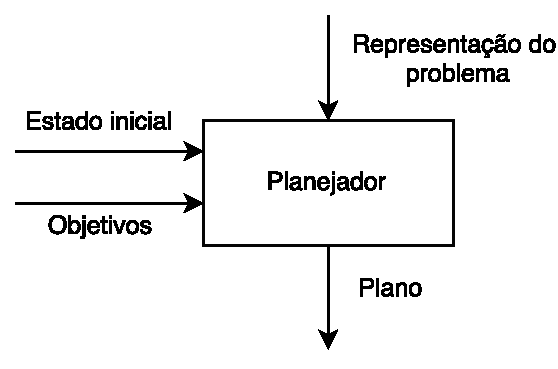
\includegraphics[width=1\textwidth]{fig/modelo.pdf}
	\caption{Modelo de estado e transição}
	\label{fig:planmodelo}
\end{figure} 


%paragrafo que introduza os dois tipos de planejamento ou somente o HTN

%\subsection{Planejamento Clássico}
%\subsection{Planejamento Neoclassico}
%**formas de planejaento\\ 
%-metodos \\
%*classico \\
%**o que é \\
%** objetivos \\
%** complexidade \\
%** limitações \\
%*neoclassico
%** o que é \\
%** tipos \\

%-definição \msr{acho que ficou desnecessario esse topico}\\

%-conceitos \cite{ghallab2004automated}\\
%**modelos(assumptions) \\


\subsection{HTN} 
-como se encaixa em planejamento \\ 
** linkar com planejamento classico\\
** difereças do planejamento classico\\
-definição \\
** o que é\\ 
** decomposição de tarefas \\
** subtask \\
** goals \\
** modelo formal \\
**diferença entre SPN e total order SPN \\
** problemas \\

-conceitos \msr{acho que ficou desnecessario esse topico}\\

\subsection{AHTN} 
-como se encaixa em planejamento e HTN \\
**o que é (HTN + game search tree)\\
** quem propos\cite{ontanon2015adversarial} \\
-definição \\
** game search tree \\
** como encaixou as duas coisas
** algoritmo \\
-conceitos \msr{acho que este topico ficou desnecessario} \\

%**Motivação \\
\subsection{Motivação e aplicação}
Uma motivação para o estudo de planejamento automatizado vem do fato que, como planejamento é um componente vital do comportamento racional, e a IA busca alcançar aspectos de inteligencia a nível computacional, então planejamento é um elemento chave para isso\cite{ghallab2004automated}.
-aplicação no mundo real\\
**como se aplica \\
**exemplo de problema \\

\section{Aprendizado} 
-overview de aprendizado
**O que é em geral \\
**o que é em computação \\
**formas de machine learning\\
**Motivação \\

\subsection{Aprendizado de Máquina} 
- overview de aprendizado de maquina \\
**
- definição \\
- conceitos

\subsection{Aprendizado por Reforço} 
\todo[color=red,author=Felipe,inline]{Pode ser desnecessário mesmo. Troca o tom do teu azul, é tri agressivo nos olhos, hehe.}
- como se encaixa dentro de aprendizado de maquina \\
** o que é \\
** tipos de learning(passivo e ativo) \\
* passivo \\
** o que é \\
** como funciona \\
** algoritmos \\
* ativo \\
** o que é \\
** como funciona \\
** algoritmos \\

%- definição \msr{acho que este topico ficou desnecessario}\\
%- conceitos \msr{acho que este topico ficou desnecessario}

\section{Jogos Real-time Strategy(RTS)} 

%Explicação do que é jogos RTS \\
%**jogos
%** RTS
%**jogos rts
Jogos eletrônicos são muito populares, não só entre os jovens, principalmente pela grande quantidade de gêneros, existem jogos de ação, aventura, esportes, estrategia, entre outros. \\
Dentro dos jogos de estratégia há uma subseção que se chama jogos de estratégia em tempo real, neles os jogadores estão se enfrentando no mesmo momento, como o nome já diz. Em alguns desses jogos há BOTs(jogadores que simulam um jogador real) e é preciso alguma inteligencia para esses BOTs conseguirem levar graça ao jogador real, para isso é utilizado algoritmos de IA. Esse tipo de jogo, devido a sua grande quantidade de ações, possui um fator de ramificação muito grande, e cresce exponencialmente, com isso aplicar os algoritmos se torna uma tarefa não trivial.  \\
%ligação deles com atividades do mundo real \\
%exemplos de jogos RTS 
Como exemplo para esse gênero de jogos foi escolhido o jogo MicroRTS para representar e ser utilizado como plataforma. 

\subsection{MicroRTS} 
%explicação de como funciona, para que foi feito. 
O jogo MicroRTS foi feito por \cite{ontanon2013combinatorial} para fins acadêmicos, com o intuito de aplicar e desenvolver técnicas de IA e para servir como prova de conceito para as técnicas criadas.  
A figura \ref{fig:jogo} mostra a tela do jogo para que se possa observar que o fator de ramificação pode ser muito alto.

\begin{figure}[ht]
	\centering
	%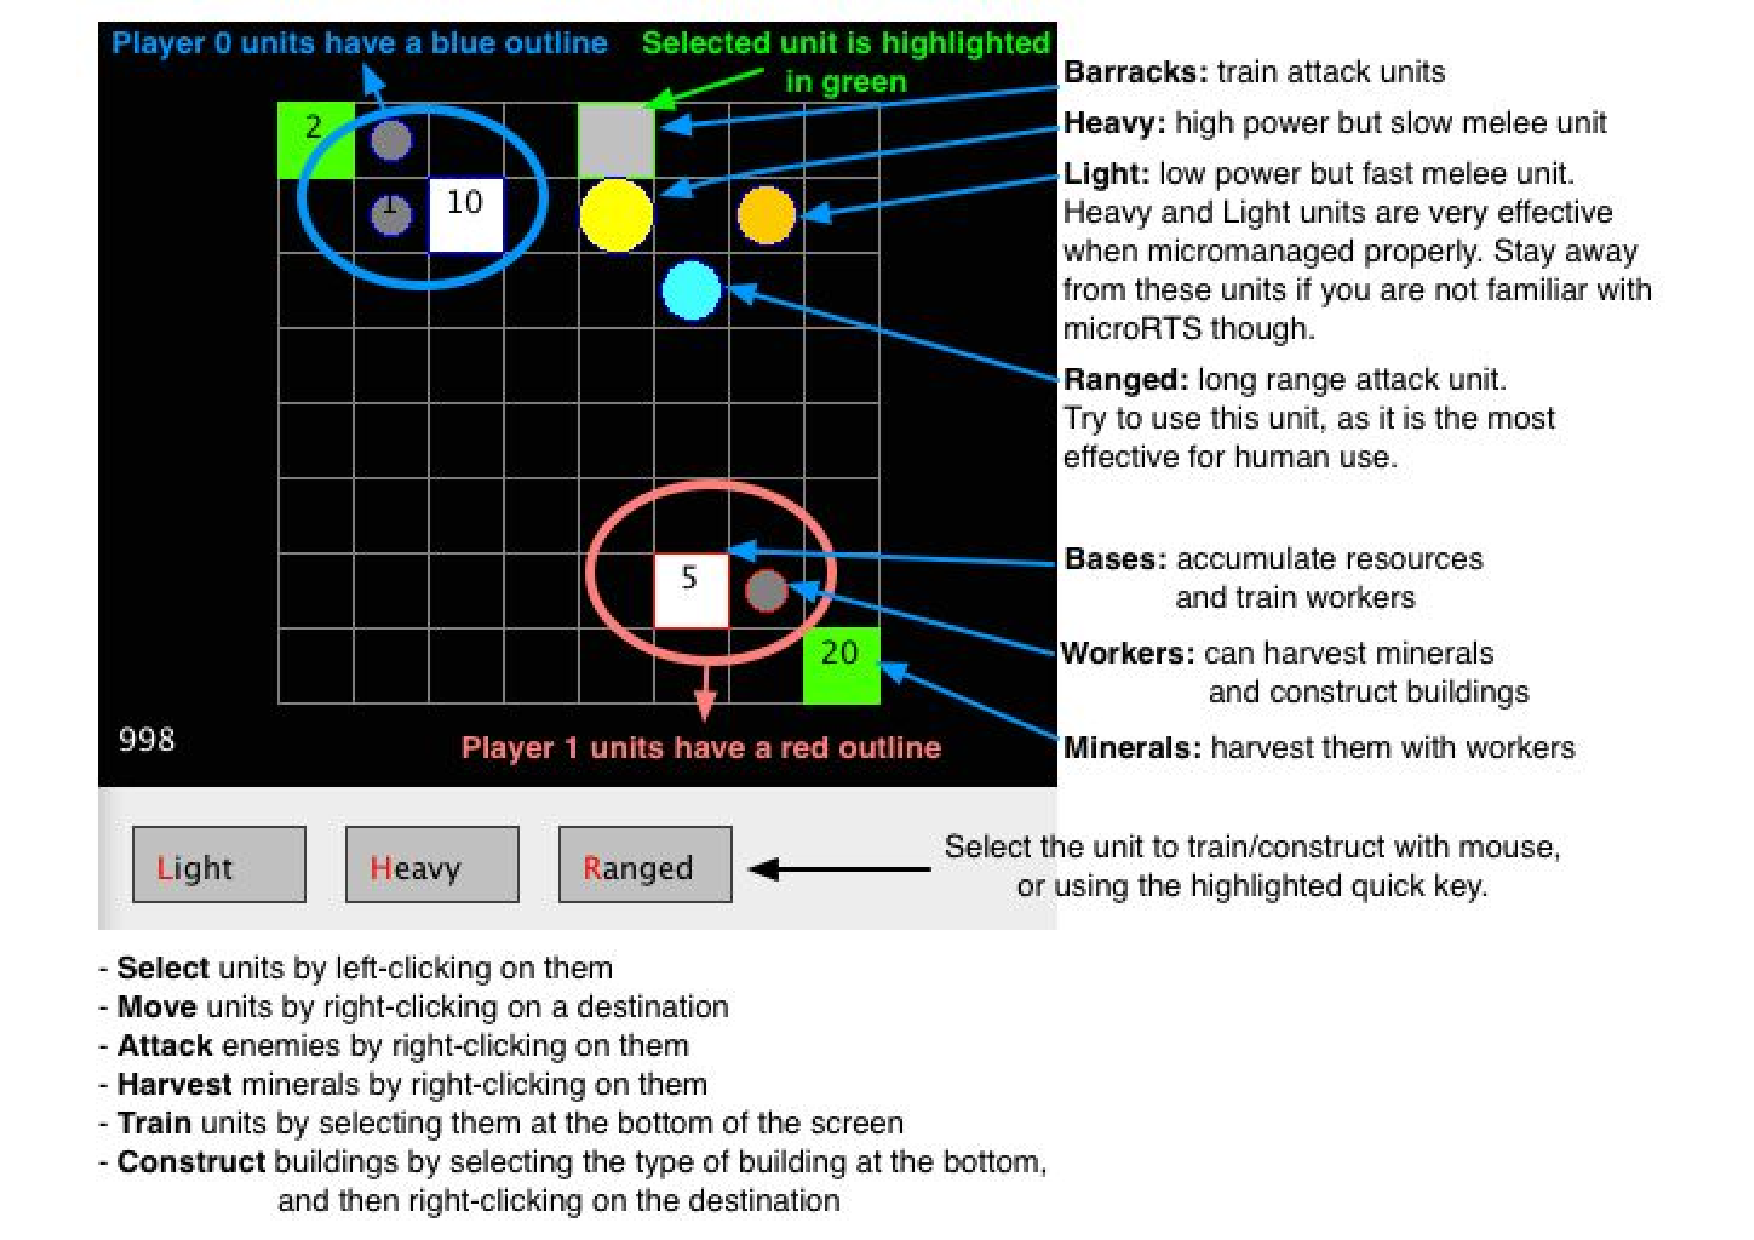
\includegraphics[width=1\textwidth]{fig/microrts.pdf}
	\caption{Uma foto da tela do MicroRTS}
	\label{fig:microrts}
\end{figure} 
